\ifx\wholebook\relax \else
% ------------------------

\documentclass{article}
%------------------- Other types of document example ------------------------
%
%\documentclass[twocolumn]{IEEEtran-new}
%\documentclass[12pt,twoside,draft]{IEEEtran}
%\documentstyle[9pt,twocolumn,technote,twoside]{IEEEtran}
%
%-----------------------------------------------------------------------------
%%
% loading packages
%
\newif\ifpdf
\ifx\pdfoutput\undefined % We're not running pdftex
  \pdffalse
\else
  \pdftrue
\fi
%
%
\ifpdf
  \RequirePackage[pdftex,%
            CJKbookmarks,%
       bookmarksnumbered,%
              colorlinks,%
          linkcolor=blue,%
              hyperindex,%
        plainpages=false,%
       pdfstartview=FitH]{hyperref}
\else
  \RequirePackage[dvipdfm,%
             CJKbookmarks,%
        bookmarksnumbered,%
               colorlinks,%
           linkcolor=blue,%
               hyperindex,%
         plainpages=false,%
        pdfstartview=FitH]{hyperref}
  \AtBeginDvi{\special{pdf:tounicode GBK-EUC-UCS2}} % GBK -> Unicode
\fi
\usepackage{hyperref}

% other packages
%-----------------------------------------------------------------------------
\usepackage{graphicx, color}
\usepackage{CJK}
%
% for programming 
%
\usepackage{verbatim}
\usepackage{listings}


\lstdefinelanguage{Smalltalk}{
  morekeywords={self,super,true,false,nil,thisContext}, % This is overkill
  morestring=[d]',
  morecomment=[s]{"}{"},
  alsoletter={\#:},
  escapechar={!},
  literate=
    {BANG}{!}1
    {UNDERSCORE}{\_}1
    {\\st}{Smalltalk}9 % convenience -- in case \st occurs in code
    % {'}{{\textquotesingle}}1 % replaced by upquote=true in \lstset
    {_}{{$\leftarrow$}}1
    {>>>}{{\sep}}1
    {^}{{$\uparrow$}}1
    {~}{{$\sim$}}1
    {-}{{\sf -\hspace{-0.13em}-}}1  % the goal is to make - the same width as +
    %{+}{\raisebox{0.08ex}{+}}1		% and to raise + off the baseline to match -
    {-->}{{\quad$\longrightarrow$\quad}}3
	, % Don't forget the comma at the end!
  tabsize=2
}[keywords,comments,strings]

\lstloadlanguages{C++, Lisp, Smalltalk}

% ======================================================================

\def\BibTeX{{\rm B\kern-.05em{\sc i\kern-.025em b}\kern-.08em
    T\kern-.1667em\lower.7ex\hbox{E}\kern-.125emX}}

\newtheorem{theorem}{Theorem}

%
% mathematics
%
\newcommand{\be}{\begin{equation}}
\newcommand{\ee}{\end{equation}}
\newcommand{\bmat}[1]{\left( \begin{array}{#1} }
\newcommand{\emat}{\end{array} \right) }
\newcommand{\VEC}[1]{\mbox{\boldmath $#1$}}

% numbered equation array
\newcommand{\bea}{\begin{eqnarray}}
\newcommand{\eea}{\end{eqnarray}}

% equation array not numbered
\newcommand{\bean}{\begin{eqnarray*}}
\newcommand{\eean}{\end{eqnarray*}}

\RequirePackage{CJK,CJKnumb,CJKulem,CJKpunct}
% we use CJK as default environment
\AtBeginDocument{\begin{CJK*}{GBK}{song}\CJKtilde\CJKindent\CJKcaption{GB}}
\AtEndDocument{\clearpage\end{CJK*}}

%
% loading packages
%
\newif\ifpdf
\ifx\pdfoutput\undefined % We're not running pdftex
  \pdffalse
\else
  \pdftrue
\fi
%
%
\ifpdf
  \RequirePackage[pdftex,%
       bookmarksnumbered,%
              colorlinks,%
          linkcolor=blue,%
              hyperindex,%
        plainpages=false,%
       pdfstartview=FitH]{hyperref}
\else
  \RequirePackage[dvipdfm,%
        bookmarksnumbered,%
               colorlinks,%
           linkcolor=blue,%
               hyperindex,%
         plainpages=false,%
        pdfstartview=FitH]{hyperref}
\fi
\usepackage{hyperref}

% other packages
%-----------------------------------------------------------------------------
\usepackage{graphicx, color}
%
% for programming 
%
\usepackage{verbatim}
\usepackage{listings}
\usepackage{algorithmic} %for pseudocode
\usepackage{algorithm}


\lstdefinelanguage{Smalltalk}{
  morekeywords={self,super,true,false,nil,thisContext}, % This is overkill
  morestring=[d]',
  morecomment=[s]{"}{"},
  alsoletter={\#:},
  escapechar={!},
  literate=
    {BANG}{!}1
    {UNDERSCORE}{\_}1
    {\\st}{Smalltalk}9 % convenience -- in case \st occurs in code
    % {'}{{\textquotesingle}}1 % replaced by upquote=true in \lstset
    {_}{{$\leftarrow$}}1
    {>>>}{{\sep}}1
    {^}{{$\uparrow$}}1
    {~}{{$\sim$}}1
    {-}{{\sf -\hspace{-0.13em}-}}1  % the goal is to make - the same width as +
    %{+}{\raisebox{0.08ex}{+}}1		% and to raise + off the baseline to match -
    {-->}{{\quad$\longrightarrow$\quad}}3
	, % Don't forget the comma at the end!
  tabsize=2
}[keywords,comments,strings]

\lstloadlanguages{C++, Lisp, Haskell, Python, Smalltalk}

% ======================================================================

\def\BibTeX{{\rm B\kern-.05em{\sc i\kern-.025em b}\kern-.08em
    T\kern-.1667em\lower.7ex\hbox{E}\kern-.125emX}}

\newtheorem{theorem}{Theorem}

%
% mathematics
%
\newcommand{\be}{\begin{equation}}
\newcommand{\ee}{\end{equation}}
\newcommand{\bmat}[1]{\left( \begin{array}{#1} }
\newcommand{\emat}{\end{array} \right) }
\newcommand{\VEC}[1]{\mbox{\boldmath $#1$}}

% numbered equation array
\newcommand{\bea}{\begin{eqnarray}}
\newcommand{\eea}{\end{eqnarray}}

% equation array not numbered
\newcommand{\bean}{\begin{eqnarray*}}
\newcommand{\eean}{\end{eqnarray*}}




\setcounter{page}{1}

\begin{document}

\fi
%--------------------------

% ================================================================
%                 COVER PAGE
% ================================================================

\title{Suffix Tree}

\author{Larry~LIU~Xinyu
\thanks{{\bfseries Larry LIU Xinyu } \newline
  Email: liuxinyu95@gmail.com \newline}
  }

\markboth{Suffix Tree}{Elementary Algorithms}

\maketitle

\ifx\wholebook\relax
\chapter{Suffix Tree}
\numberwithin{Exercise}{chapter}
\fi

%{\bfseries Corresponding Author:} Larry LIU Xinyu

% ================================================================
%                 Introduction
% ================================================================
\section{Introduction}
\label{introduction}

Suffix Tree is an important data structure.
It can be used to realize many important string operations particularly
fast\cite{wiki-suffix-tree}. It is
also widely used in bio-information area such as DNA pattern
matching\cite{ukkonen-presentation}.
Weiner introduced suffix tree in 1973\cite{weiner73}.
The latest on-line construction algorithm was found in 1995\cite{ukkonen95}.

The suffix tree for a string $S$ is a special Patricia.
Each edge is labeled with some sub-string of $S$.
Each suffix of $S$ corresponds to exactly one path
from the root to a leaf. Figure \ref{fig:stree-banana} shows the suffix tree for
English word `banana'.

\begin{figure}[htbp]
  \centering
  \includegraphics[scale=0.5]{img/stree-banana.ps}
  \caption{The suffix tree for `banana'} \label{fig:stree-banana}
\end{figure}

All suffixes, 'banana', 'anana', 'nana', 'ana', 'na', 'a', '' can
be found in the above tree. Among them the first 3 suffixes are explicitly
shown; others are implicitly represented. The reason for why 'ana, 'na', 'a',
and '' are not shown is because they are prefixes of the others.
In order to show all suffixes explicitly, we can append a special pad
terminal symbol, which doesn't occur in other places in the string.
Such terminator is typically
denoted as '\$'. By this means, there is no suffix being the prefix of the others.

Although the suffix tree for 'banana' is simple, the
suffix tree for 'bananas', as shown in figure \ref{fig:stree-bananas}, is quite different.

\begin{figure}[htbp]
  \centering
  \includegraphics[scale=0.5]{img/stree-bananas.ps}
  \caption{The suffix tree for `bananas'} \label{fig:stree-bananas}
\end{figure}

To create suffix suffix tree for a given string, we can utilize the
insertion algorithmS explained in previous chatper for Patricia.

\begin{algorithmic}[1]
\Function{Suffix-Tree}{$S$}
  \State $T \gets$ NIL
  \For{$i \gets 1$ to $|S|$}
    \State $T \gets$ \textproc{Patricia-Insert}($T$, \Call{Right}{$S, i$})
  \EndFor
  \State \Return $T$
\EndFunction
\end{algorithmic}

For non-empty string $S=s_1s_2...s_i...s_n$ of length $n = |S|$, function
\textproc{Right}($S, i$) $= s_is_{i+1...s_n}$. It extracts the sub-string of $S$
from the $i$-th character to the last one. This straightforward algorithm
can also be defined as below.

\be
suffix_T(S) = fold(insert_{patricia}, \Phi, suffixes(S))
\ee

Where function $suffixes(S)$ gives all the suffixes for string $S$. If
the string is empty, the result is one empty string; otherwise, $S$
itself is one suffix, the others can be given by recursively call
$suffixes(S')$, where $S'$ is given by drop the first character from $S$.

\be
suffixes(S) = \left \{
  \begin{array}
  {r@{\quad:\quad}l}
  \{ \Phi \} & S = \Phi \\
  \{S\} \cup suffixes(S') & otherwise
  \end{array}
\right.
\ee

This solution constructs suffix tree in $O(n^2)$ time, for string of length $n$.
It totally inserts $n$ suffixes to the tree, and each
insertion takes linear time proportion to the length of the suffix.
The efficiency isn't good enough.

In this chapter, we firstly explain a fast on-line suffix trie construction
solution by using suffix link concpet. Because trie isn't space efficient,
we next introduce a linear time on-line suffix tree construction algorithm
found by Ukkonen. and show
how to solve some interesting string manipulation problems with
suffix tree.

% ================================================================
%                 Suffix Trie
% ================================================================
\section{Suffix trie}
\label{suffix-trie}
\index{Suffix trie}

Just likes the relationship between trie and Patricia, Suffix trie has much simpler
structure than suffix tree. Figure \ref{fig:strie-banana} shows the suffix trie for
'banana'.

\begin{figure}[htbp]
  \centering
  \includegraphics[scale=0.4]{img/strie-banana.ps}
  \caption{Suffix trie for 'banana'} \label{fig:strie-banana}
\end{figure}

Compare with figure \ref{fig:stree-banana}, we can find the difference between
suffix tree and suffix trie. Instead of representing
a word, every edge in suffix trie only represents a character.
Thus suffix trie needs much more spaces.
If we pack all nodes which have only one child, the suffix
trie is turned into a suffix tree.

We can reuse the trie definition for suffix tree. Each node is bound to a
character, and contains mutiple sub trees as children. A child can be
refered from the bounded character.

% ================================================================
%               Online construction of Suffix Trie
% ================================================================
\subsection{Node transfer and suffix link}

For string $S$ of length $n$, define $S_i=s_1s_2...s_i$.
It is the prefix contains the first $i$ characters.

\index{Suffix tree!node transfer}
In suffix trie, each node represents a suffix string. for example in figure
\ref{fig:strie-cacao}, node $X$ represents suffix 'a', by adding character 'c',
node $X$ transfers to $Y$ which represents suffix 'ac'. We say node $X$ transfer
to $Y$ with the edge of character 'c'\cite{ukkonen95}.

\begin{figure}[htbp]
  \centering
  \includegraphics[scale=0.45]{img/strie-cacao.ps}
  \caption{Suffix trie for string ``cacao''. Node $X \gets$ ``a'', node $Y \gets$ ``ac'', $X$ transfers to $Y$ with character 'c'}
  \label{fig:strie-cacao}
\end{figure}

\begin{algorithmic}
\State $Y \gets$ \Call{Children}{$X$}[$c$]
\end{algorithmic}

We also say that node $X$ has a 'c'-child $Y$. Below Python expression
reflects this concept.

\lstset{language=python}
\begin{lstlisting}
y = x.children[c]
\end{lstlisting}

\index{Suffix link}
If node $A$ in a suffix trie represents suffix $s_is_{i+1}...s_n$,
and node $B$ represents suffix $s_{i+1}s_{i+2}...s_n$, we say node $B$
represents {\em the suffix} of node $A$. We can create a link from $A$ to $B$.
This link is defined as {\em the suffix link} of node $A$\cite{ukkonen95}.
Suffix link is drawn in dotted style. In figure \ref{fig:strie-cacao}, the suffix link of
node $A$ points to node $B$, and the suffix link of node $B$ points to node $C$.

Suffix link is valid for all nodes except the root. We can add a suffix link field to
the trie definition. Below Python example code shows this update.

\lstset{language=Python}
\begin{lstlisting}
class STrie:
    def __init__(self, suffix=None):
        self.children = {}
        self.suffix = suffix
\end{lstlisting}

\subsection{On-line construction}

For string $S$, Suppose we have constructed suffix trie for the $i$-th prefix
$S_i=s_1s_2...s_i$. Denote it as $SuffixTrie(S_i)$.
Let's consider how to obtain $SuffixTrie(S_{i+1})$ from $SuffixTrie(S_i)$.

If list all suffixes corresponding to $SuffixTrie(S_i)$, from the longest
(which is $S_i$) to the shortest (which is empty), we can get
table \ref{tab:suffixes_s_i}. There are total $i+1$ suffixes.

\begin{table}
  \begin{tabular}{r}
    suffix string \\
    $s_1s_2s_3...s_i$ \\
    $s_2s_3...s_i$ \\
    ... \\
    $s_{i-1}s_i$ \\
    $s_i$ \\
    ``'' \\
  \end{tabular}
  \caption{suffixes for $S_i$}
  \label{tab:suffixes_s_i}
\end{table}

One solution is to append the character $s_{i+1}$ to every suffix in this
table, then add another empty string. This idea can be realized by adding
a new child for every node in the trie, and binding all these new
child with edge of character $s_{i+1}$.

\begin{algorithm}
\begin{algorithmic}[1]
\For{$\forall T \in SuffixTrie(S_i)$}
  \State \Call{Children}{$T$}[$s_{i+1}$] $\gets$ \Call{Create-Empty-Node}{}
\EndFor
\end{algorithmic}
\caption{Update $SuffixTrie(S_i)$ to $SuffixTrie(S_{i+1})$, initial version.}
\label{algo:strie1}
\end{algorithm}

However, some nodes in $SuffixTrie(S_i)$ may have the $s_{i+1}$-child already.
For example, in figure \ref{fig:strie-cac}, node $X$ and $Y$ are corresponding
for suffix 'cac' and 'ac' respectively. They don't have the 'a'-child.
But node $Z$, which represents suffix 'c' has the 'a'-child already.

\begin{figure}[htbp]
  \centering
  \subfloat[Suffix trie for string ``cac''.]{\hspace{.2\textwidth}\includegraphics[scale=0.5]{img/strie-cac.ps}\hspace{.2\textwidth}}
  \subfloat[Suffix trie for string ``caca''.]{\hspace{.2\textwidth}\includegraphics[scale=0.5]{img/strie-caca.ps}\hspace{.2\textwidth}}
  \caption{Suffix Trie of ``cac'' and ``caca''}
  \label{fig:strie-cac}
\end{figure}

When append $s_{i+1}$ to $SuffixTrie(S_i)$. In this example $s_{i+1}$ is character 'a'.
We need create new nodes for $X$ and $Y$, but we needn't do this
for $Z$.

If check the nodes one by one according to table \ref{tab:suffixes_s_i}, we can
stop immediately when meet a node which has the $s_{i+1}$-child. This is because
if node $X$ in $SuffixTrie(S_i)$ has the $s_{i+1}$-child, according to the
definition of suffix link, any suffix nodes $X'$ of $X$ in $SuffixTrie(S_i)$ must
also have the $s_{i+1}$-child. In other words, let $c=s_{i+1}$, if $wc$ is a sub-string
of $S_i$, then every suffix of $wc$ is also a sub-string of $S_i$ \cite{ukkonen95}.
The only exception is the root, which represents for empty string ``''.

According to this fact, we can refine the algorithm \ref{algo:strie1} to
the following.

\begin{algorithm}
  \begin{algorithmic}[1]
  \For{each $T \in SuffixTrie(S_i)$ in descending order of suffix length}
    \If{\Call{Children}{$T$}[$s_{i+1}$] = NIL}
      \State \Call{Children}{$T$}[$s_{i+1}$] $\gets$ \Call{Create-Empty-Node}{}
    \Else
      \State break
    \EndIf
  \EndFor
  \end{algorithmic}
  \caption{Update $SuffixTrie(S_i)$ to $SuffixTrie(S_{i+1})$, second version.}
  \label{algo:strie2}
\end{algorithm}

The next question is how to iterate all nodes
in descending order of the suffix length? Define the {\em top} of a suffix
trie as the deepest leaf node. This definition ensures the top represents
the longest suffix. Along the suffix link from the top to the next node,
the length of the suffix decrease by one. This fact tells us that
We can traverse the suffix tree from the top
to the root by using the suffix links. And the order of such traversing
is exactly what we want.
Finally, there is a special suffix trie for empty string $SuffixTrie(NIL)$,
We define the top equals to the root in this case.

\begin{algorithmic}
\Function{Insert}{$top, c$}
  \If{$top = $ NIL} \Comment{The trie is empty}
    \State $top \gets$ \Call{Create-Empty-Node}{}
  \EndIf
  \State $T \gets top$
  \State $T' \gets$ \Call{Create-Empty-Node}{} \Comment{dummy init value}
  \While{$T \neq$ NIL $\land$ \Call{Children}{$T$}[$c$] = NIL}
    \State \Call{Children}{$T$}[$c$] $\gets$ \Call{Create-Empty-Node}{}
    \State \Call{Suffix-Link}{$T'$} $\gets$ \Call{Children}{$T$}[$c$]
    \State $T' \gets$ \Call{Children}{$T$}[$c$]
    \State $T \gets$ \Call{Suffix-Link}{$T$}
  \EndWhile
  \If{$T \neq$ NIL}
    \State \Call{Suffix-Link}{$T'$} $\gets$ \Call{Children}{$T$}[$c$]
  \EndIf
  \State \Return \Call{Children}{$top$}[$c$] \Comment{returns the new top}
\EndFunction
\end{algorithmic}

Function \textproc{Insert}, updates $SuffixTrie(S_i)$ to $SuffixTrie(S_{i+1})$.
It takes two arguments, one is the top of $SuffixTrie(S_i)$, the other
is $s_{i+1}$ character. If the top is NIL, it means the tree is empty,
so there is no root. The algorithm creates a root node in this case.
A sentinel empty node $T'$ is created. It keeps tracking the previous
created new node. In the main loop, the algorithm checks every node
one by one along the suffix link. If the node hasn't the $s_{i+1}$-child,
it then creates a new node, and binds the edge to character $s_{i+1}$.
The algorithm repeatedly goes up along the suffix link until either
arrives at the root, or find a node which has the $s_{i+1}$-child already.
After the loop, if the node isn't empty, it means we stop at a node
which has the $s_{i+1}$-child.
The last suffix link then points to that child.
Finally, the new top position is returned, so that we can futher
insert other characters to the suffix trie.

For a given string $S$, the suffix trie can be built by repeatedly
calling \textproc{Insert} function.

\begin{algorithmic}[1]
\Function{Suffix-Trie}{$S$}
  \State $t \gets$ NIL
  \For{$i \gets 1$ to $|S|$}
    \State $t \gets$ \Call{Insert}{$t, s_i$}
  \EndFor
  \State \Return $t$
\EndFunction
\end{algorithmic}

This algorithm returns the top of the suffix trie, but not the root.
In order to access the root, we can traverse along the suffix link.

\begin{algorithmic}[1]
\Function{Root}{$T$}
  \While{\Call{Suffix-Link}{$T$} $\neq$ NIL}
    \State $T \gets$ \Call{Suffix-Link}{$T$}
  \EndWhile
  \State \Return $T$
\EndFunction
\end{algorithmic}

Figure \ref{fig:cons-strie-cacao} shows the steps
when construct suffix trie for ``cacao''.
Only the last layer of suffix links are shown.

\begin{figure}[htbp]
  \centering
  \subfloat[Emtpy]{\hspace{.1\textwidth}\includegraphics[scale=0.5]{img/strie-empty.ps}\hspace{.1\textwidth}}
  \subfloat[``c'']{\hspace{.1\textwidth}\includegraphics[scale=0.5]{img/strie-c.ps}\hspace{.1\textwidth}}
  \subfloat[``ca'']{\hspace{.1\textwidth}\includegraphics[scale=0.5]{img/strie-ca.ps}\hspace{.1\textwidth}} \\
  \subfloat[``cac'']{\hspace{.1\textwidth}\includegraphics[scale=0.5]{img/strie-cac.ps}\hspace{.1\textwidth}}
  \subfloat[``caca'']{\hspace{.1\textwidth}\includegraphics[scale=0.5]{img/strie-caca.ps}\hspace{.1\textwidth}}
  \subfloat[``cacao'']{\hspace{.1\textwidth}\includegraphics[scale=0.5]{img/strie-cacao.ps}\hspace{.1\textwidth}}
  \caption{Construct suffix trie for ``cacao''. There are 6 steps. Only the last layer of suffix links are shown in dotted arrow.}
  \label{fig:cons-strie-cacao}
\end{figure}

For \textproc{Insert} algorihtm, the computation time
is proportion to the size of suffix trie. In the worse case, the suffix trie is
built in $O(n^2)$ time, where $n = |S|$. One example is $S=a^nb^n$, that there are $n$
characters of $a$ and $n$ characters of $b$.

The following example Python program implements the suffix trie construction algorithm.

\lstset{language=Python}
\begin{lstlisting}
def suffix_trie(str):
    t = None
    for c in str:
        t = insert(t, c)
    return root(t)

def insert(top, c):
    if top is None:
        top=STrie()
    node = top
    new_node = STrie() #dummy init value
    while (node is not None) and (c not in node.children):
        new_node.suffix = node.children[c] = STrie(node)
        new_node = node.children[c]
        node = node.suffix
    if node is not None:
        new_node.suffix = node.children[c]
    return top.children[c] #update top

def root(node):
    while node.suffix is not None:
        node = node.suffix
    return node
\end{lstlisting}

% ================================================================
%               Suffix Tree
% ================================================================
\section{Suffix Tree}
\index{Suffix tree}

Suffix trie isn't space efficient, and the construction time
is quadratic. If don't care about the speed, we can compress the
suffix trie to suffix tree\cite{trivial-stree-java}. Ukkonen
found a linear time on-line suffix tree construction algorithm
in 1995.

% ================================================================
%               Online construction of suffix tree
% ================================================================
\subsection{On-line construction}

\subsubsection{Active point and end point}
\label{ap-and-ep}
\index{Suffix tree!active point}
\index{Suffix tree!end point}

The suffix trie construction algorithm shows very
important fact about what happens when $SuffixTrie(S_i)$ updates to
$SuffixTrie(S_{i+1})$. Let's review the last two steps in figure
\ref{fig:cons-strie-cacao}.

There are two different updates.
\begin{enumerate}
\item All leaves are appended with a new node for $s_{i+1}$;
\item Some non-leaf nodes are branched out with a new node for $s_{i+1}$.
\end{enumerate}

The first type of update is trivial, because for all new coming characters,
we need do this work anyway. Ukkonen defines leaf as the 'open' node.

The second type of update is important. We need figure out which internal
nodes need branch out. We only focus on these nodes and apply the
update.

Ukkonen defines the path along the suffix links from the top to the end
as 'boundary path'.
Denote the nodes in boundary path  as, $n_1, n_2, ..., n_j, ..., n_k$.
These nodes start from the leaf node (the first one is the top position),
suppose that after the $j$-th node, they are not leaves any longer,
we need repeatedly branch out from this time point till the $k$-th node.

Ukkonen defines the first none-leaf node $n_j$ as 'active point' and the last
node $n_k$ as 'end point'. The end point can be the root.

\subsubsection{Reference pair}
\index{Suffix tree!reference pair}

\begin{figure}[htbp]
  \centering
  \includegraphics[scale=0.5]{img/stree-bananas-label.ps}
  \caption{Suffix tree of ``bananas''. $X$ transfer to $Y$ with sub-string ``na''.}
  \label{fig:stree-bananas-label}
\end{figure}

Figure \ref{fig:stree-bananas-label} shows the suffix tree of English word ``bananas''.
Node $X$ represents suffix ``a''. By adding sub-string ``na'', node $X$ transfers
to node $Y$, which represents suffix ``ana''.
In other words, we can
represent $Y$ with a pair of node and sub-string, like $(X, w)$, where $w=$ ``na''.
Ukkonen defines
such kind of pair as {\em reference pair}. Not only the explicit node, but also the
implicit position in suffix tree can be represented with reference pair. For example,
$(X$, ``n'' $)$ represents to a position which is not an explicit node. By using reference
pair, we can represent every position in a suffix tree.

In order to save spaces, for string $S$, all sub-strings can
be represented as a pair of index $(l, r)$, where $l$ is the left index and $r$ is the
right index of the character for the sub-string. For instance, if $S=$ ``bananas'', and the
index starts from 1, sub-string ``na'' can be represented with pair $(3, 4)$. As the result,
there is only one copy of the complete string, and all positions in the suffix tree
is defined as $(node, (l, r))$. This is the final form of reference pair.

With reference pair, node transfer for suffix tree can be defined as the following.

\textproc{Children}($X$)[$s_l$] $\gets ((l, r), Y) \iff Y \gets (X, (l, r))$

If character $s_l=c$, we say that node $X$ has a $c$-child, This child is $Y$.
$Y$ can be transfered from $X$ with sub string $(l, r)$
Each node can have at most one $c$-child.

\subsubsection{canonical reference pair}

It's obvious that the one position in a suffix tree may have multiple reference pairs.
For example, node $Y$ in Figure \ref{fig:stree-bananas-label} can be either
denoted as $(X, (3, 4))$ or $(root, (2, 4))$. If we define empty string
$\epsilon=(i, i-1)$, $Y$ can also be represented as $(Y, \epsilon)$.

The canonical reference pair is the one which has the closest node
to the position. Specially, in case the position is an
explicit node, the canonical reference pair is $(node, \epsilon)$, so $(Y, \epsilon)$
is the canonical reference pair of node $Y$.

Below algorithm converts a reference pair $(node, (l, r))$
to the canonical reference pair $(node', (l', r))$.
Note that since $r$ doesn't change, the algorithm can only return
$(node', l')$ as the result.

\begin{algorithm}
\begin{algorithmic}[1]
\Function{Canonize}{$node, (l, r)$}
  \If{$node = $ NIL}
    \If{$(l, r) = \epsilon$}
      \State \Return $($ NIL, $l)$
    \Else
      \State \Return \Call{Canonize}{$root, (l+1, r)$}
    \EndIf
  \EndIf
  \While{$l \leq r$} \Comment{$(l, r) isn't empty $}
    \State $((l', r'), node') \gets$ \Call{Children}{$node$}[$s_l$]
    \If{$ r-l \geq r'-l'$}
      \State $l \gets l + r' - l' + 1$ \Comment{Remove $|(l', r')|$ chars from $(l, r)$}
      \State $node \gets node'$
    \Else
      \State break
    \EndIf
  \EndWhile
  \State \Return $(node, l)$
\EndFunction
\end{algorithmic}
\caption{Convert reference pair to canonical reference pair}
\label{algo:canon}
\end{algorithm}

If the passed in node parameter is NIL, it means a very special case.
The function is called like the following.

\textproc{Canonize}(\textproc{Suffix-Link}($root$), $(l, r)$)

Because the suffix link of root points to NIL, the result should be
$(root, (l+1, r))$ if $(l, r)$ is not $\epsilon$. Otherwise,
$($NIL, $\epsilon)$ is returned to indicate a terminal position.

We explain this special case in detail in later sections.

\subsubsection{The algorithm}

In \ref{ap-and-ep}, we mentioned, all updating to leaves is trivial, because we
only need append the new coming character to the leaf. With reference pair,
it means, when update $SuffixTree(S_i)$ to $SuffixTree(S_{i+1})$,
all reference pairs in form $(node, (l, i))$, are leaves. They will
change to $(node, (l, i+1))$ next time. Ukkonen defines leaf in form
$(node, (l, \infty))$, here $\infty$ means ``open to grow''. We can skip all
leaves until the suffix tree is completely constructed. After that, we can
change all $\infty$ to the length of the string.

So the main algorithm only cares about {\em positions} from the active point
to the end point. However, how to find the active point and the end point?

When start suffix tree construction, there is only a root node. There aren't
any branches or leaves. The active point should be $(root, \epsilon)$, or
$(root, (1, 0))$ (the string index starts from 1).

For the end point, it is a position where we can finish updating $SuffixTree(S_i)$.
According to the suffix trie algorithm, we know it should be a
{\em position} which has the $s_{i+1}$-child already. Because a position
in suffix trie may not be an explicit node in suffix tree, if $(node, (l, r))$
is the end point, there are two cases.

\begin{enumerate}
\item $(l, r)=\epsilon$. It means the node itself is the end point. This node has the
$s_{i+1}$-child, which means \textproc{Children}($node$)[$s_{i+1}$] $\neq$ NIL;
\item Otherwise, $l \leq r$, the end point is an implicit position.
It must satisfy $s_{i+1}=s_{l'+|(l, r)|}$, where
\textproc{Children}($node$)[$s_l$]$=((l', r'), node')$, $|(l, r)|$ means
the length of sub-string $(l, r)$. It equals to $r-l+1$.
This is illustrated in figure \ref{fig:implicit-end-point}. We can
also say that $(node, (l, r))$ has a $s_{i+1}$-child implicitly.
\end{enumerate}

\begin{figure}[htbp]
  \centering
  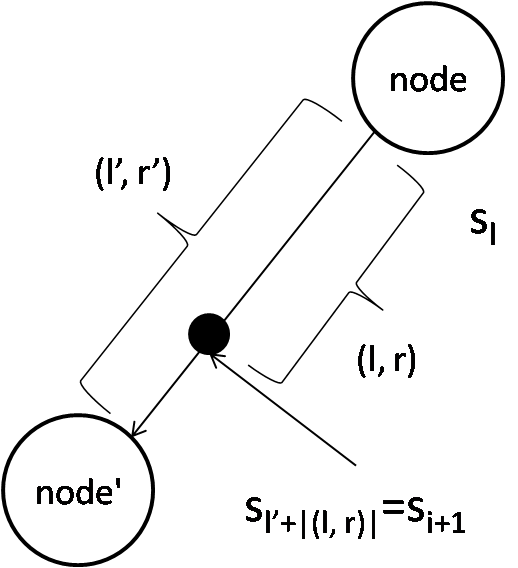
\includegraphics[scale=0.5]{img/implicit-end-point.eps}
  \caption{Implicit end point}
  \label{fig:implicit-end-point}
\end{figure}

Ukkonen finds a very important fact that if $(node, (l, i))$ is the end
point of $SuffixTree(S_i)$, then $(node, (l, i+1))$ is the active point of
$SuffixTree(S_{i+1})$.

This is because if $(node, (l, i))$ is the end point of $SuffixTree(S_i)$,
it must have a $s_{i+1}$-child (either explicitly or implicitly).
If this end point represents suffix $s_ks_{k+1}...s_i$, it is the longest
suffix in $SuffxiTree(S_i)$ which satisfies $s_ks_{k+1}...s_is_{i+1}$ is a sub-string
of $S_i$. Consider $S_{i+1}$, $s_ks_{k+1}...s_is_{i+1}$ must occur at least
twice in $S_{i+1}$, so position $(node, (l, i+1))$ is the active point of
$SuffixTree(S_{i+1})$. Figure \ref{fig:ep-ap} shows about this truth.

\begin{figure}[htbp]
  \centering
  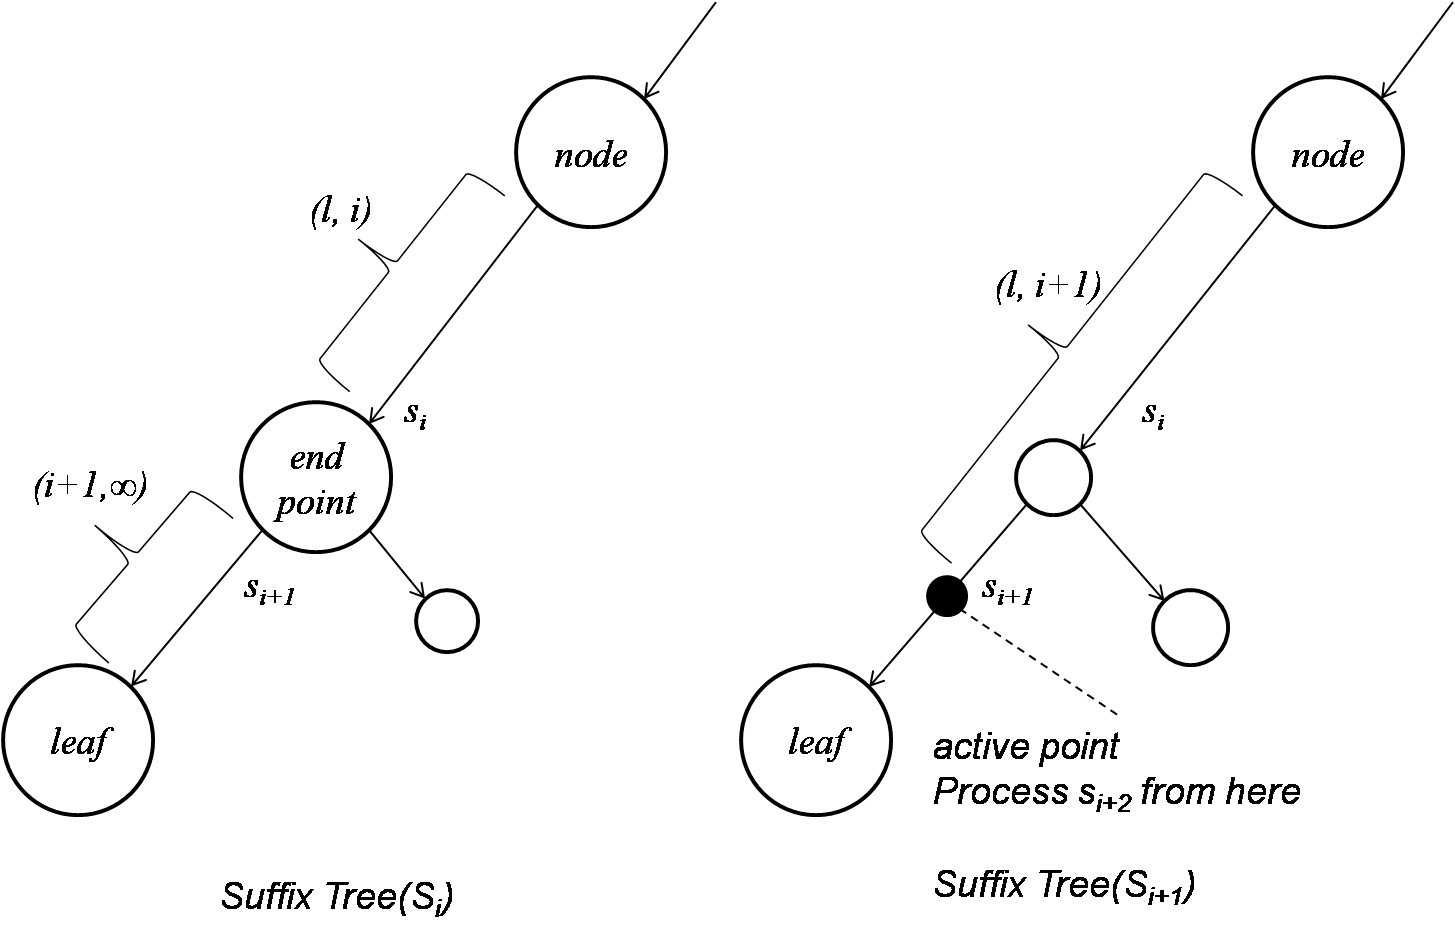
\includegraphics[scale=0.5]{img/ep-ap.eps}
  \caption{End point in $SuffixTree(S_i)$ and active point in $SuffixTree(S_{i+1})$.}
  \label{fig:ep-ap}
\end{figure}

Summarize the above facts, the algorithm of Ukkonen's on-line construction can
be given as the following.

%\begin{algorithm}
\begin{algorithmic}[1]
\Function{Update}{$node, (l, i)$}
  \State $prev \gets$ \Call{Create-Empty-Node}{} \Comment{Initilized as sentinel} %
  \Loop \Comment{Traverse along the suffix links}
    \State $(finish, node') \gets$ \Call{End-Point-Branch?}{$node, (l, i-1), s_i$}
    \If{$finish$}
      \State break
    \EndIf
    \State \Call{Children}{$node'$}[$s_i$] $\gets$ ($(i, \infty)$, \Call{Create-Empty-Node}{})
    \State \Call{Suffix-Link}{$prev$} $\gets node'$
    \State $prev \gets node'$
    \State $(node, l) = $ \textproc{Canonize}(\Call{Suffix-Link}{$node$}, $(l, i-1)$)
  \EndLoop
  \State \Call{Suffix-Link}{$prev$} $\gets node$
  \State \Return $(node, l)$ \Comment{The end point}
\EndFunction
\end{algorithmic}
%\caption{Update $SuffixTree(S_{i-1})$}
%\label{algo:update}
%\end{algorithm}

This algorithm takes reference pair $(node, (l, i))$ as arguments, note that
position $(node, (l, i-1)$ is the active point for $SuffixTree(S_{i-1})$.
Then we start a loop, this loop goes along the suffix links until
the current position $(node, (l, i-1))$ is the end point. Otherwise,
function \textproc{End-Point-Branch?} returns a position, from
where the new leaf branch out.

The \textproc{End-Point-Branch?} algorithm is realized as below.

%\begin{algorithm}
\begin{algorithmic}
\Function{End-Point-Branch?}{$node, (l, r), c$}
  \If{$(l, r) = \epsilon$}
    \If{$node = $ NIL}
      \State \Return (TRUE, $root$)
    \Else
      \State \Return (\Call{Children}{$node$}[$c$] = NIL, $node$)
    \EndIf
  \Else
    \State $((l', r'), node') \gets$ \Call{Children}{$node$}[$s_l$]
    \State $pos \gets l' + |(l, r)|$
    \If{$s_{pos} = c$}
      \State \Return (TRUE, $node$)
    \Else
      \State $p \gets$ \Call{Create-Empty-Node}{}
      \State \Call{Children}{$node$}[$s_{l'}$] $\gets ((l', pos-1), p)$
      \State \Call{Children}{$p$}[$s_{pos}$] $\gets ((pos, r'), node')$
      \State \Return (FALSE, $p$)
    \EndIf
  \EndIf
\EndFunction
\end{algorithmic}
%\caption{Test if a position is end point and create explicit node for further branching.}
%\label{algo:branch}
%\end{algorithm}

If the position is $(root, \epsilon)$, it means we have arrived at the root.
It's definitely the end point, so that we can finish this round of updating.
If the position is in form of $(node, \epsilon)$, it means the reference pair represents
an explicit node, we can examine if this node has already the $c$-child, where $c=s_i$.
If not, we need branch out a leaf.

Otherwise, the position $(node, (l, r))$ points to an implicit node.
We need find the exact position next to it to see if there is a $c$-child.
If yes, we meet an end point, the updating loop can be finished; else, we turn
the position to an explicit node, and return it for further branching.

We can finalize the Ukkonen's algorithm as below.

%\begin{algorithm}
\begin{algorithmic}[1]
\Function{Suffix-Tree}{$S$}
  \State $root \gets$ \Call{Create-Empty-Node}{}
  \State $node \gets root, l \gets 0$
  \For{$i \gets 1$ to $|S|$}
    \State $(node, l) = $ \Call{Update}{$node, (l, i)$}
    \State $(node, l) = $ \Call{Canonize}{$node, (l, i)$}
  \EndFor
  \State \Return $root$
\EndFunction
\end{algorithmic}
%\caption{Main algorithm of Ukkonen's on-line construction for suffix tree.}
%\label{algo:ukkonen2}
%\end{algorithm}

Figure \ref{fig:cons-stree-cacao} shows the steps when constructing the
suffix tree for string ``cacao''.

\begin{figure}[htbp]
  \centering
  \subfloat[Empty]{\hspace{.1\textwidth}\includegraphics[scale=0.5]{img/strie-empty.ps}\hspace{.1\textwidth}}
  \subfloat[``c'']{\hspace{.1\textwidth}\includegraphics[scale=0.5]{img/stree-c.ps}\hspace{.1\textwidth}}
  \subfloat[``ca'']{\hspace{.1\textwidth}\includegraphics[scale=0.5]{img/stree-ca.ps}\hspace{.1\textwidth}} \\
  \subfloat[``cac'']{\hspace{.1\textwidth}\includegraphics[scale=0.5]{img/stree-cac.ps}\hspace{.1\textwidth}}
  \subfloat[``caca'']{\hspace{.1\textwidth}\includegraphics[scale=0.5]{img/stree-caca.ps}\hspace{.1\textwidth}}
  \subfloat[``cacao'']{\hspace{.1\textwidth}\includegraphics[scale=0.5]{img/stree-cacao.ps}\hspace{.1\textwidth}}
  \caption{Construct suffix tree for ``cacao''. There are 6 steps. Only the last layer of suffix links are shown in dotted arrow.}
  \label{fig:cons-stree-cacao}
\end{figure}

Note that we needn't set suffix link for leaf nodes, only branch nodes
need suffix links.

The following example Python program implements Ukkonen's algorithm.
First is the node definition.

\lstset{language=Python}
\begin{lstlisting}
class Node:
    def __init__(self, suffix=None):
        self.children = {} # 'c':(word, Node), where word = (l, r)
        self.suffix = suffix
\end{lstlisting}

Because there is only one copy of the complete string, all sub-strings
are represent in $(left, right)$ pairs, and the leaf are open pairs
as $(left, \infty)$. The suffix tree is defined like below.

\begin{lstlisting}
class STree:
    def __init__(self, s):
        self.str = s
        self.infinity = len(s)+1000
        self.root = Node()
\end{lstlisting}

The infinity is defined as the length of the string plus a big number.
Some auxiliar functions are definded.

\begin{lstlisting}
def substr(str, str_ref):
    (l, r)=str_ref
    return str[l:r+1]

def length(str_ref):
    (l, r)=str_ref
    return r-l+1
\end{lstlisting}

The main entry for Ukkonen's algorithm is implemented as the following.

\begin{lstlisting}
def suffix_tree(str):
    t = STree(str)
    node = t.root # init active point is (root, Empty)
    l = 0
    for i in range(len(str)):
        (node, l) = update(t, node, (l, i))
        (node, l) = canonize(t, node, (l, i))
    return t

def update(t, node, str_ref):
    (l, i) = str_ref
    c = t.str[i] # current char
    prev = Node() # dummy init
    while True:
        (finish, p) = branch(t, node, (l, i-1), c)
        if finish:
            break
        p.children[c]=((i, t.infinity), Node())
        prev.suffix = p
        prev = p
        (node, l) = canonize(t, node.suffix, (l, i-1))
    prev.suffix = node
    return (node, l)

def branch(t, node, str_ref, c):
    (l, r) = str_ref
    if length(str_ref)<=0: # (node, empty)
        if node is None: #_|_
            return (True, t.root)
        else:
            return ((c in node.children), node)
    else:
        ((l1, r1), node1) = node.children[t.str[l]]
        pos = l1+length(str_ref)
        if t.str[pos]==c:
            return (True, node)
        else:
            branch_node = Node()
            node.children[t.str[l1]]=((l1, pos-1), branch_node)
            branch_node.children[t.str[pos]] = ((pos, r1), node1)
            return (False, branch_node)

def canonize(t, node, str_ref):
    (l, r) = str_ref
    if node is None:
        if length(str_ref)<=0:
            return (None, l)
        else:
            return canonize(t, t.root, (l+1, r))
    while l<=r: # str_ref is not empty
        ((l1, r1), child) = node.children[t.str[l]]
        if r-l >= r1-l1:
            l += r1-l1+1
            node = child
        else:
            break
    return (node, l)
\end{lstlisting}

\subsubsection{Functional suffix tree construction}

Giegerich and Kurtz found Ukkonen's algorithm
can be transformed to McCreight's algorithm\cite{GieKur97}.
The three suffix tree construction algorithms found by
Weiner, McCreight, and Ukkonen are all bound to $O(n)$ time.
Giegerich and Kurtz conjectured any sequential
suffix tree construction method doesn't base on
suffix links, active suffixes, etc., fails to meet the
$O(n)$-criterion.

There is implementation in PLT/Scheme\cite{plt-stree} based on
Ukkonen's algorithm, However, it updates suffix links during the
processing, which is not purely functional.

A lazy suffix tree construction method is discussed in \cite{GieKur95}.
And this method is contributed to Haskell Hackage by Bryan O'Sullivan.
\cite{Hackage-STree}. The method depends on the lazy evaluation property.
The tree won't be constructed until it is traversed.
However, it can't ensure the $O(n)$ performance
if the programming environments or languages don't support
lazy evalutation.

The following Haskell program defines the suffix tree. A suffix tree
is either a leaf, or a branch containing mulitple sub trees. Each
sub tree is bound to a string.

\lstset{language=Haskell}
\begin{lstlisting}
data Tr = Lf | Br [(String, Tr)] deriving (Eq)
type EdgeFunc = [String]->(String, [String])
\end{lstlisting}

The edge function extracts a common prefix from a list of strings.
The prefix returned by edge function may not be the longest one,
empty string is also allowed. The exact behavior can be customized
with different edge functions.

\begin{lstlisting}
lazyTree::EdgeFunc -> [String] -> Tr
lazyTree edge = build where
    build [[]] = Lf
    build ss = Br [(a:prefix, build ss') |
                         a<-alpha,
                         xs@(x:_) <-[[cs | c:cs<-ss, c==a]],
                         (prefix, ss')<-[edge xs]]
\end{lstlisting}

\begin{lstlisting}
alpha = ['a'..'z']++['A'..'Z']
\end{lstlisting}

lazyTree function takes a list of string, it will generate a radix
tree (for example a Trie or a Patricia) from these string.

It will categorize all strings with the first letter in several groups,
and remove the first letter for each elements in every group.
For example, for the string list [``acac'', ``cac'', ``ac'', ``c'']
the categorized group will be [('a', [``cac'', ``c'']), ('c', [``ac'', ``''])].
For easy understanding, I left the first letter, and write the groups
as tuple. then all strings with same first letter (removed) will
be fed to edge function.

Different edge function produce different radix trees. The most trivial
one will build a Trie.

\begin{lstlisting}
edgeTrie::EdgeFunc
edgeTrie ss = ("", ss)
\end{lstlisting}

If the edge function extract the longest common prefix, then it will
build a Patricia.

\begin{lstlisting}
-- ex:
--   edgeTree ["an", "another", "and"] = ("an", ["", "other", "d"])
--   edgeTree ["bool", "foo", "bar"] = ("", ["bool", "foo", "bar"])
--
-- some helper comments
--   let awss@((a:w):ss) = ["an", "another", "and"]
--       (a:w) = "an",  ss = ["another", "and"]
--       a='a', w="n"
--       rests awss = w:[u| _:u<-ss] = ["n", "nother", "nd"]
--
edgeTree::EdgeFunc
edgeTree [s] = (s, [[]])
edgeTree awss@((a:w):ss) | null [c|c:_<-ss, a/=c] = (a:prefix, ss')
                         | otherwise              = ("", awss)
                         where (prefix, ss') = edgeTree (w:[u| _:u<-ss])
edgeTree ss = ("", ss) -- (a:w):ss can't be match <==> head ss == ""
\end{lstlisting}

We can build suffix Trie and suffix tree with the above two functions.

\begin{lstlisting}
suffixTrie::String->Tr
suffixTrie = lazyTree edgeTrie . tails -- or init . tails

suffixTree::String->Tr
suffixTree = lazyTree edgeTree . tails
\end{lstlisting}

Function lazyTree is common for all radix trees, the normal Patricia
and Trie can also be constructed with it.

\begin{lstlisting}
trie::[String]->Tr
trie = lazyTree edgeTrie

patricia::[String]->Tr
patricia = lazyTree edgeTree
\end{lstlisting}

% ================================================================
%               Suffix tree applications
% ================================================================

\section{Suffix tree applications}

Suffix tree can help to solve a lot of string/DNA manipulation problems
particularly fast. For typical problems will be list in this section.

\subsection{String/Pattern searching}
\label{substring-lookup}

There a plenty of string searching problems, among them includes the
famous KMP algorithm. Suffix tree can perform same level as
KMP\cite{zhang-shaojie-lec}, that string searching in $O(m)$ complexity,
where $m$ is the length of the sub-string.However, O(n) time is
required to build the suffix tree in advance\cite{lallison-stree}.

Not only sub-string searching, but also pattern matching, including
regular expression matching can be solved with suffix tree. Ukkonen
summarize this kind of problems as sub-string motifs, and he gave the
result that {\em For a string $S$, $SuffixTree(S)$ gives complete occurrence
counts of all sub-string motifs of $S$ in $O(n)$ time, although $S$ may have
$O(n^2)$ sub-strings.}

Note the facts of a $SuffixTree(S)$ that all internal nodes is corresponding
to a repeating sub-string of $S$ and the number of leaves of the sub-tree of a
node for string $P$ is the number of occurrence of $P$ in $S$.\cite{ukkonen-lec}

\subsubsection{Algorithm of finding the number of sub-string occurrence}
The algorithm is almost as same as the Patricia looking up algorithm,
please refer to \cite{lxy-trie} for detail, the only difference is that
the number of the children is returned when a node matches the pattern.

\subsubsection*{Find number of sub-string occurrence in Python}

In Ukkonen's algorithm, there is only one copy
of string, and all edges are represent with index pairs. There are
some changes because of this reason.

\lstset{language=Python}
\begin{lstlisting}
def lookup_pattern(t, node, s):
    f = (lambda x: 1 if x==0 else x)
    while True:
        match = False
        for _, (str_ref, tr) in node.children.items():
            edge = t.substr(str_ref)
            if string.find(edge, s)==0: #s `isPrefixOf` edge
                return f(len(tr.children))
            elif string.find(s, edge)==0: #edge `isPrefixOf` s
                match = True
                node = tr
                s = s[len(edge):]
                break
        if not match:
            return 0
    return 0 # not found
\end{lstlisting}

In case a branch node matches the pattern, it means there is at least
one occurrence even if the number of children is zero. That's why
a local lambda function is defined.

I added a member function in STree to convert a string index
pair to string as below.

\begin{lstlisting}
class STree:
    #...
    def substr(self, sref):
        return substr(self.str, sref)
\end{lstlisting}

In lookup\_pattern() function, it takes a suffix tree which
is built from the string.
A node is passed as the position to be looked up, it is root node when
starting. Parameter s is the string to be searched.

The algorithm iterate all children of the node, it convert the string
index reference pair to edge sub-string, and check if s is prefix of the
the edge string, if matches, then the program can be terminated, the
number of the branches of this node will be returned as the number
of the occurrence of this sub-string. Note that no branch means there
is only 1 occurrence. In case the edge is prefix of s, we then
updated the node and string to be searched and go on the searching.

Because construction of the suffix tree is expensive, so we only
do it when necessary. We can do a lazy initialization as below.

\begin{lstlisting}
TERM1 = '$' # $: special terminator

class STreeUtil:
    def __init__(self):
        self.tree = None

    def find_pattern(self, str, pattern):
        if self.tree is None or self.tree.str!=str+TERM1:
            self.tree = stree.suffix_tree(str+TERM1)
        return lookup_pattern(self.tree, self.tree.root, pattern)
\end{lstlisting}

We always append special terminator to the string, so that there won't
be any suffix becomes the prefix of the other\cite{wiki-suffix-tree}.

Some simple test cases are given to verify the program.

\begin{lstlisting}
class StrSTreeTest:
    def run(self):
        self.test_find_pattern()

    def test_find_pattern(self):
        util=STreeUtil()
        self.__test_pattern__(util, "banana", "ana")
        self.__test_pattern__(util, "banana", "an")
        self.__test_pattern__(util, "banana", "anan")
        self.__test_pattern__(util, "banana", "nana")
        self.__test_pattern__(util, "banana", "ananan")

    def __test_pattern__(self, u, s, p):
        print "find pattern", p, "in", s, ":", u.find_pattern(s, p)
\end{lstlisting}

And the output is like the following.

\begin{verbatim}
find pattern ana in banana : 2
find pattern an in banana : 2
find pattern anan in banana : 1
find pattern nana in banana : 1
find pattern ananan in banana : 0
\end{verbatim}

\subsubsection*{Find the number of sub-string occurrence in C++}
In C++, do-while is used as the repeat-until structure, the program
is almost as same as the standard Patricia looking up function.

\lstset{language=C++}
\begin{lstlisting}
int lookup_pattern(const STree* t, std::string s){
  Node* node = t->root;
  bool match(false);
  do{
    match=false;
    for(Node::Children::iterator it = node->children.begin();
        it!=node->children.end(); ++it){
      RefPair rp = it->second;
      if(rp.str().substr().find(s)==0){
        int res = rp.node()->children.size();
        return res == 0? 1 : res;
      }
      else if(s.find(rp.str().substr())==0){
        match = true;
        node = rp.node();
        s = s.substr(rp.str().substr().length());
        break;
      }
    }
  }while(match);
  return 0;
}
\end{lstlisting}

An utility class is defined and it support lazy initialization to save
the cost of construction of suffix tree.

\begin{lstlisting}
class STreeUtil{
public:
  STreeUtil():t(0){}
  ~STreeUtil(){ delete t; }

  int find_pattern(std::string s, std::string pattern){
    lazy(s);
    return lookup_pattern(t, pattern);
  }
private:
  void lazy(std::string s){
    if((!t) || t->str != s+TERM1){
      delete t;
      t = suffix_tree(s+TERM1);
    }
  }
  STree* t;
};
\end{lstlisting}

The same test cases can be feed to this C++ program.

\begin{lstlisting}
class StrSTreeTest{
public:
  void test_find_pattern(){
    __test_pattern("banana", "ana");
    __test_pattern("banana", "an");
    __test_pattern("banana", "anan");
    __test_pattern("banana", "nana");
    __test_pattern("banana", "ananan");
  }
pivate:
  void __test_pattern(std::string s, std::string ptn){
    std::cout<<"find pattern "<<ptn<<" in "<<s<<": "
             <<util.find_pattern(s, ptn)<<"\n";
  }

  STreeUtil util;
};
\end{lstlisting}

And the same result will be obtained like the Python program.

\subsubsection*{Find the number of sub-string occurrence in Haskell}
The Haskell program is just turn the looking up into recursive way.

\lstset{language=Haskell}
\begin{lstlisting}
lookupPattern :: Tr -> String -> Int
lookupPattern (Br lst) ptn = find lst where
    find [] = 0
    find ((s, t):xs)
         | ptn `isPrefixOf` s = numberOfBranch t
         | s `isPrefixOf` ptn = lookupPattern t (drop (length s) ptn)
         | otherwise = find xs
    numberOfBranch (Br ys) = length ys
    numberOfBranch _ = 1

findPattern :: String -> String -> Int
findPattern s ptn = lookupPattern (suffixTree $ s++"$") ptn
\end{lstlisting}

To verify it, the test cases are fed to the program as the following
\begin{lstlisting}
testPattern = ["find pattern "++p++" in banana: "++
               (show $ findPattern "banana" p)
                   | p<- ["ana", "an", "anan", "nana", "anana"]]
\end{lstlisting} %$

Launching GHCi, evaluate the instruction can output the same result
as the above programs.

\begin{lstlisting}
 putStrLn $ unlines testPattern
\end{lstlisting} %$

\subsubsection*{Find the number of sub-string occurrence in Scheme/Lisp}
Because the underground data structure of suffix tree is list in
Scheme/Lisp program, we needn't define a inner find function as
in Haskell program.

\lstset{language=lisp}
\begin{lstlisting}
(define (lookup-pattern t ptn)
  (define (number-of-branches node)
    (if (null? node) 1 (length node)))
  (if (null? t) 0
      (let ((s (edge (car t)))
	    (tr (children (car t))))
	(cond ((string-prefix? ptn s)(number-of-branches tr))
	      ((string-prefix? s ptn)
	       (lookup-pattern tr (string-tail ptn (string-length s))))
	      (else lookup-pattern (cdr t) ptn)))))
\end{lstlisting}

The test cases are fed to this program via a list.

\begin{lstlisting}
(define (test-pattern)
  (define (test-ptn t s)
    (cons (string-append "find pattern " s " in banana" )
	  (lookup-pattern t s)))
  (let ((t (suffix-tree "banana")))
    (map (lambda (x) (test-ptn t x)) '("ana" "an" "anan" "nana" "anana"))))
\end{lstlisting}

Evaluate this test function can generate a result list as the following.
\begin{lstlisting}
(test-pattern)
;Value 16: (("find pattern ana in banana" . "ana") ("find pattern an in banana" . "an") ("find pattern anan in banana" . "anan") ("find pattern nana in banana" . "nana") ("find pattern anana in banana" . "anana"))
\end{lstlisting}

\subsubsection{Complete pattern search}
For search pattern like ``a**n'' with suffix tree, please refer to \cite{ukkonen-lec} and \cite{ukkonen-search}.

\subsection{Find the longest repeated sub-string}

If we go one step ahead from \ref{substring-lookup}, below result can
be found.

{\em After adding a special terminator character to string S, The
longest repeated sub-string can be found by searching the
deepest branches in suffix tree.}

Consider the example suffix tree shown in figure \ref{fig:stree-mississippis}

\begin{figure}[htbp]
   \begin{center}
      \includegraphics[scale=0.5]{img/stree-mississippis.ps}
      \caption{The suffix tree for `mississippi\$'} \label{fig:stree-mississippis}
   \end{center}
\end{figure}

There are 3 branch nodes, A, B, and C which depth is 3. However, A represents
the longest repeated sub-string ``issi''. B and C represent for ``si'', ``ssi'',
they are all shorter than A.

This example tells us that the ``depth'' of the branch node should be measured
by the number of characters traversed from the root.

\subsubsection{Find the longest repeated sub-string in imperative approach}
According to the above analysis, to find the longest repeated sub-string
can be turned into a BFS (Bread First Search) in a suffix tree.

\begin{algorithmic}[1]
\Function{LONGEST-REPEATED-SUBSTRING}{$T$}
  \State $Q \leftarrow (NIL, ROOT(T))$
  \State $R \leftarrow NIL$
  \While{$Q$ is not empty}
    \State $(s, node) \leftarrow POP(Q)$
    \For{each $((l, r), node')$ in $CHILDREN(node)$}
      \If{$node'$ is not leaf}
        \State $s' \leftarrow CONCATENATE(s, (l, r))$
        \State $PUSH(Q, (s', node'))$
        \State $UPDATE(R, s')$
      \EndIf
    \EndFor
  \EndWhile
  \State \Return $R$
\EndFunction
\end{algorithmic}

where algorithm $UPDATE()$ will compare the longest repeated sub-string
candidates. If two candidates have the same length, one simple solution
is just take one as the final result, the other solution is to maintain
a list contains all candidates with same length.

\begin{algorithmic}[1]
\Function{UPDATE}{$l, x$}
  \If{$l = NIL$ or $LENGTH(l[1]) < LENGTH(x)$}
    \State \Return $l \leftarrow [x]$
  \ElsIf {$LENGTH(l[1]) = LENGTH(x)$}
    \State \Return $APPEND(l, x)$
  \EndIf
\EndFunction
\end{algorithmic}

Note that the index of a list starts from 1 in this algorithm.
This algorithm will first initialize a queue with a pair of an
empty string and the root node. Then it will repeatedly pop from
the queue, examine the candidate node until the queue is empty.

For each node, the algorithm will expand all children, if it is
a branch node (which is not a leaf), the node will be pushed back
to the queue for future examine. And the sub-string represented
by this node will be compared to see if it is a candidate of the
longest repeated sub-string.

\subsubsection*{Find the longest repeated sub-string in Python}
The above algorithm can be translated into Python program as the following.

\lstset{language=Python}
\begin{lstlisting}
def lrs(t):
    queue = [("", t.root)]
    res = []
    while len(queue)>0:
        (s, node) = queue.pop(0)
        for _, (str_ref, tr) in node.children.items():
            if len(tr.children)>0:
                s1 = s+t.substr(str_ref)
                queue.append((s1, tr))
                res = update_max(res, s1)
    return res

def update_max(lst, x):
    if lst ==[] or len(lst[0]) < len(x):
        return [x]
    elif len(lst[0]) == len(x):
        return lst + [x]
    else:
        return lst
\end{lstlisting}

In order to verify this program, some simple test cases are fed.

\begin{lstlisting}
class StrSTreeTest:
    #...

    def run(self):
        #...
        self.test_lrs()

    def test_lrs(self):
        self.__test_lrs__("mississippi")
        self.__test_lrs__("banana")
        self.__test_lrs__("cacao")
        self.__test_lrs__("foofooxbarbar")

    def __test_lrs__(self, s):
        print "longest repeated substrings of", s, "=", self.util.find_lrs(s)
\end{lstlisting}

By running the test case, the result like below can be obtained.

\begin{verbatim}
longest repeated substrings of mississippi = ['issi']
longest repeated substrings of banana = ['ana']
longest repeated substrings of cacao = ['ca']
longest repeated substrings of foofooxbarbar = ['bar', 'foo']
\end{verbatim}

\subsubsection*{Find the longest repeated sub-string in C++}
With C++, we can utilize the STL queue library in the implementation
of BFS(Bread First Search).

\lstset{language=C++}
\begin{lstlisting}
typedef std::list<std::string> Strings;

Strings lrs(const STree* t){
  std::queue<std::pair<std::string, Node*> > q;
  Strings res;
  q.push(std::make_pair(std::string(""), t->root));
  while(!q.empty()){
    std::string s;
    Node* node;
    tie(s, node) = q.front();
    q.pop();
    for(Node::Children::iterator it = node->children.begin();
        it!=node->children.end(); ++it){
      RefPair rp = it->second;
      if(!(rp.node()->children.empty())){
        std::string s1 = s + rp.str().substr();
        q.push(std::make_pair(s1, rp.node()));
        update_max(res, s1);
      }
    }
  }
  return res;
}
\end{lstlisting}

Firstly, the empty string and root node is pushed to the queue
as initialized value. Then the program repeatedly pop from the queue,
examine it to see if any child of the node is not a leaf node,
push it back to the queue and check if it is the deepest one.

The function ``update\_max()'' is implemented to record all the
longest strings.

\begin{lstlisting}
void update_max(Strings& res, std::string s){
  if(res.empty() || (*res.begin()).length() < s.length()){
    res.clear();
    res.push_back(s);
    return;
  }
  if((*res.begin()).length() == s.length())
    res.push_back(s);
}
\end{lstlisting}

Since the cost of construction a suffix tree is big ($O(n)$ with
Ukkonen's algorithm), some lazy initialization approach is used in
the main entrance of the finding program.

\begin{lstlisting}
const char TERM1 = '$';

class STreeUtil{
public:
  STreeUtil():t(0){}
  ~STreeUtil(){ delete t; }

  Strings find_lrs(std::string s){
    lazy(s);
    return lrs(t);
  }

private:
  void lazy(std::string s){
    if((!t) || t->str != s+TERM1){
      delete t;
      t = suffix_tree(s+TERM1);
    }
  }
  STree* t;
};
\end{lstlisting} %$

In order to verify the program, some test cases are provided. output
for list of strings can be easily realized by overloading ``operator<<''.

\begin{lstlisting}
class StrSTreeTest{
public:
  StrSTreeTest(){
    std::cout<<"start string manipulation over suffix tree test\n";
  }

  void run(){
    test_lrs();
  }

  void test_lrs(){
    __test_lrs("mississippi");
    __test_lrs("banana");
    __test_lrs("cacao");
    __test_lrs("foofooxbarbar");
  }
private:
  void __test_lrs(std::string s){
    std::cout<<"longest repeated substirng of "<<s<<"="
             <<util.find_lrs(s)<<"\n";
  }
  STreeUtil util;
};
\end{lstlisting}

Running these test cases, we can obtain the following result.
\begin{verbatim}
start string manipulation over suffix tree test
longest repeated substirng of mississippi=[issi, ]
longest repeated substirng of banana=[ana, ]
longest repeated substirng of cacao=[ca, ]
longest repeated substirng of foofooxbarbar=[bar, foo, ]
\end{verbatim}

\subsubsection{Find the longest repeated sub-string in functional approach}
Searching the deepest branch can also be realized in functional way.
If the tree is just a leaf node, empty string is returned, else the
algorithm will try to find the longest repeated sub-string from the
children of the tree.

\begin{algorithmic}[1]
\Function{LONGEST-REPEATED-SUBSTRING'}{$T$}
  \If{$T$ is leaf}
    \State \Return $Empty$
  \Else
    \State \Return $PROC(CHILDREN(T))$
  \EndIf
\EndFunction
\end{algorithmic}

\begin{algorithmic}[1]
\Function{PROC}{$L$}
  \If{$L$ is empty}
    \State \Return $Empty$
  \Else
    \State $(s, node) \leftarrow FIRST(L)$
    \State $x \leftarrow s + LONGEST-REPEATED-SUBSTRING'(T)$
    \State $y \leftarrow PROC(REST(L))$
    \If{$LENGTH(x) > LENGTH(y)$}
      \State \Return $x$
    \Else
      \State \Return $y$
    \EndIf
  \EndIf
\EndFunction
\end{algorithmic}

In $PROC$ function, the first element, which is a pair of edge string
and a child node, will be examine firstly. We recursively call the
algorithm to find the longest repeated sub-string from the child node,
and append it to the edge string. Then we compare this candidate
sub string with the result obtained from the rest of the children.
The longer one will be returned as the final result.

Note that in case $x$ and $y$ have the same length, it is easy to
modify the program to return both of them.

\subsubsection*{Find the longest repeated sub-string in Haskell}
We'll provide 2 versions of Haskell implementation. One version
just returns the first candidate in case there are multiple sub-strings
which have the same length as the longest sub-string. The other
version returns all possible candidates.

\lstset{language=Haskell}
\begin{lstlisting}
isLeaf::Tr -> Bool
isLeaf Lf = True
isLeaf _ = False

lrs'::Tr->String
lrs' Lf = ""
lrs' (Br lst) = find $ filter (not . isLeaf . snd) lst where
    find [] = ""
    find ((s, t):xs) = maximumBy (compare `on` length) [s++(lrs' t), find xs]
\end{lstlisting} %$

In this version, we used the maximumBy function provided in Data.List
module. it will only return the first maximum value in a list.
In order to return all maximum candidates, we need provide a customized
function.

\begin{lstlisting}
maxBy::(Ord a)=>(a->a->Ordering)->[a]->[a]
maxBy _ [] = []
maxBy cmp (x:xs) = foldl maxBy' [x] xs where
    maxBy' lst y = case cmp (head lst) y of
                     GT -> lst
                     EQ -> lst ++ [y]
                     LT -> [y]

lrs::Tr->[String]
lrs Lf = [""]
lrs (Br lst) = find $ filter (not . isLeaf . snd) lst where
    find [] = [""]
    find ((s, t):xs) = maxBy (compare `on` length)
                             ((map (s++) (lrs t)) ++ (find xs))
\end{lstlisting} %$

We can feed some simple test cases and compare the results of
these 2 different program to see their difference.

\begin{lstlisting}
testLRS s = "LRS(" ++ s ++ ")=" ++ (show $ lrs $ suffixTree (s++"$")) ++ "\n"

testLRS' s = "LRS'(" ++ s ++ ")=" ++ (lrs' $ suffixTree (s++"$")) ++ "\n"


test = concat [ f s | s<-["mississippi", "banana", "cacao", "foofooxbarbar"],
                      f<-[testLRS, testLRS']]
\end{lstlisting} %$

Below are the results printed out.

\begin{verbatim}
LRS(mississippi)=["issi"]
LRS'(mississippi)=issi
LRS(banana)=["ana"]
LRS'(banana)=ana
LRS(cacao)=["ca"]
LRS'(cacao)=ca
LRS(foofooxbarbar)=["bar","foo"]
LRS'(foofooxbarbar)=foo
\end{verbatim}

\subsubsection*{Find the longest repeated sub-string in Scheme/Lisp}
Because the underground data structure is list in Scheme/Lisp,
in order to access the suffix tree components easily, some helper
functions are provided.

\lstset{language=lisp}
\begin{lstlisting}
(define (edge t)
  (car t))

(define (children t)
  (cdr t))

(define (leaf? t)
  (null? (children t)))
\end{lstlisting}

Similar with the Haskell program, a function which can find all
the maximum values on a special measurement rules are given.

\begin{lstlisting}
(define (compare-on func)
  (lambda (x y)
    (cond ((< (func x) (func y)) 'lt)
	  ((> (func x) (func y)) 'gt)
	  (else 'eq))))

(define (max-by comp lst)
  (define (update-max xs x)
    (case (comp (car xs) x)
      ('lt (list x))
      ('gt xs)
      (else (cons x xs))))
  (if (null? lst)
      '()
      (fold-left update-max (list (car lst)) (cdr lst))))
\end{lstlisting}

Then the main function for searching the longest repeated sub-strings
can be implemented as the following.

\begin{lstlisting}
(define (lrs t)
  (define (find lst)
    (if (null? lst)
	'("")
	(let ((s (edge (car lst)))
	      (tr (children (car lst))))
	  (max-by (compare-on string-length)
		  (append
		   (map (lambda (x) (string-append s x)) (lrs tr))
		   (find (cdr lst)))))))
  (if (leaf? t)
      '("")
      (find (filter (lambda (x) (not (leaf? x))) t))))

(define (longest-repeated-substring s)
  (lrs (suffix-tree (string-append s TERM1))))
\end{lstlisting}

Where TERM1 is defined as ``\$'' string.

Same test cases can be used to verify the results.

\begin{lstlisting}
(define (test-main)
  (let ((fs (list longest-repeated-substring))
	(ss '("mississippi" "banana" "cacao" "foofooxbarbar")))
    (map (lambda (f) (map f ss)) fs)))
\end{lstlisting}

This test program can be easily extended by adding new test
functions as a element of fs list. the result of the above
function is as below.

\begin{lstlisting}
(test-main)
;Value 16: ((("issi") ("ana") ("ca") ("bar" "foo")))
\end{lstlisting}

\subsection{Find the longest common sub-string}
The longest common sub-string of two strings, can also be quickly found
by using suffix tree. A typical solution is to build a generalized suffix
tree for two strings. If the two strings are denoted as $txt_1$ and
$txt_2$, a generalized suffix tree is $SuffixTree(txt_1\$_1txt_2\$_2)$.
Where $\$_1$ is a special terminator character for $txt_1$, and
$\$_2$ is another special terminator character for $txt_2$.

The longest common sub-string is indicated by the deepest branch node, with
two forks corresponding to both ``...$\$_1$...'' and ``...$\$_2$''(no $\$_1$).
The definition of the {\em deepest} node is as same as the one for
the longest repeated sub-string, it is the number of characters traversed
from root.

If a node has ``...$\$_1$...'' beneath it, then the node must represent
to a sub-string of $txt_1$, as $\$_1$ is the terminator of $txt_1$.
On the other hand, since it also has ``...$\$_2$'' (without $\$_1$) child, this node
must represent to a sub-string of $txt_2$ too. Because of it's a deepest
one satisfied this criteria. The node indicates to the longest common
sub-string.

\subsubsection{Find the longest common sub-string imperatively}
Based on the above analysis, a BFS (bread first search) algorithm
can be used to find the longest common sub-string.

\begin{algorithmic}[1]
\Function{LONGEST-COMMON-SUBSTRING}{$T$}
  \State $Q \leftarrow (NIL, ROOT(T))$
  \State $R \leftarrow NIL$
  \While{$Q$ is not empty}
    \State $(s, node) \leftarrow POP(Q)$
    \If{$MATCH-FORK(node)$}
      \State $UPDATE(R, s)$
    \EndIf
    \For{each $((l, r), node')$ in $CHILDREN(node)$}
      \If{$node'$ is not leaf}
        \State $s' \leftarrow CONCATENATE(s, (l, r))$
        \State $PUSH(Q, (s', node'))$
      \EndIf
    \EndFor
  \EndWhile
  \State \Return $R$
\EndFunction
\end{algorithmic}

The most part is as same as the algorithm for finding the longest repeated
sub-sting. The function $MATCH-FORK()$ will check if the children of a
node satisfy the common sub-string criteria.

\subsubsection*{Find the longest common sub-string in Python}
By translate the imperative algorithm in Python, the following program can
be obtained.

\lstset{language=Python}
\begin{lstlisting}
def lcs(t):
    queue = [("", t.root)]
    res = []
    while len(queue)>0:
        (s, node) = queue.pop(0)
        if match_fork(t, node):
            res = update_max(res, s)
        for _, (str_ref, tr) in node.children.items():
            if len(tr.children)>0:
                s1 = s + t.substr(str_ref)
                queue.append((s1, tr))
    return res
\end{lstlisting}

Where we define the function match\_fork() as below.

\begin{lstlisting}
def is_leaf(node):
    return node.children=={}

def match_fork(t, node):
    if len(node.children)==2:
        [(_, (str_ref1, tr1)), (_, (str_ref2, tr2))]=node.children.items()
        return is_leaf(tr1) and is_leaf(tr2) and \
            (t.substr(str_ref1).find(TERM2)!=-1) != \
            (t.substr(str_ref2).find(TERM2)!=-1)
    return False
\end{lstlisting}

In this function, it checks if the two children of a node
are both leaf, and one contains TERM2 character, while the
other doesn't. This is because
if one child node is a leaf, it will always contains TERM1
character according to the definition of suffix tree.

Note, the main interface of the function is to add TERM2 to
the first string and append TERM1 to the second string.

\begin{lstlisting}
class STreeUtil:
    def __init__(self):
        self.tree = None

    def __lazy__(self, str):
        if self.tree is None or self.tree.str!=str+TERM1:
            self.tree = stree.suffix_tree(str+TERM1)

    def find_lcs(self, s1, s2):
        self.__lazy__(s1+TERM2+s2)
        return lcs(self.tree)
\end{lstlisting}

We can test this program like below:

\begin{lstlisting}
util = STreeUtil()
print "longest common substring of ababa and baby =", util.find_lcs("ababa", "baby")
\end{lstlisting}

And the output will be something like:
\begin{verbatim}
longest common substring of ababx and baby = ['bab']
\end{verbatim}

\subsubsection*{Find the longest common sub-string in C++}
In C++ implementation, we first define the special terminator
characters for the generalized suffix tree of two strings.

\lstset{language=C++}
\begin{lstlisting}
const char TERM1 = '$';
const char TERM2 = '#';
\end{lstlisting} %$

Since the program need frequently test if a node is a branch
node or leaf node, a helper function is provided.

\begin{lstlisting}
bool is_leaf(Node* node){
  return node->children.empty();
}
\end{lstlisting}

The criteria for a candidate node is that it has two children.
One in pattern ``...\#...'', the other in pattern ``...\$''.

\begin{lstlisting}
bool match_fork(Node* node){
  if(node->children.size() == 2){
    RefPair rp1, rp2;
    Node::Children::iterator it = node->children.begin();
    rp1 = (it++)->second;
    rp2 = it->second;
    return (is_leaf(rp1.node()) && is_leaf(rp2.node())) &&
      (rp1.str().substr().find(TERM2)!=std::string::npos)!=
      (rp2.str().substr().find(TERM2)!=std::string::npos);
  }
  return false;
}
\end{lstlisting}

The main program in BFS(Bread First Search) approach is given
as below.

\begin{lstlisting}
Strings lcs(const STree* t){
  std::queue<std::pair<std::string, Node*> > q;
  Strings res;
  q.push(std::make_pair(std::string(""), t->root));
  while(!q.empty()){
    std::string s;
    Node* node;
    tie(s, node) = q.front();
    q.pop();
    if(match_fork(node))
      update_max(res, s);
    for(Node::Children::iterator it = node->children.begin();
        it!=node->children.end(); ++it){
      RefPair rp = it->second;
      if(!is_leaf(rp.node())){
        std::string s1 = s + rp.str().substr();
        q.push(std::make_pair(s1, rp.node()));
      }
    }
  }
  return res;
}
\end{lstlisting}

After that we can finalize the interface in a lazy way as the following.

\begin{lstlisting}
class STreeUtil{
public:
  //...
  Strings find_lcs(std::string s1, std::string s2){
    lazy(s1+TERM2+s2);
    return lcs(t);
  }
//...
\end{lstlisting}

This C++ program can generate similar result as the Python one if same
test cases are given.

\begin{verbatim}
longest common substring of ababa, baby =[bab, ]
\end{verbatim}

\subsubsection{Find the longest common sub-string recursively}
The longest common sub-string finding algorithm can also be
realized in functional way.

\begin{algorithmic}[1]
\Function{LONGEST-COMMON-SUBSTRING'}{$T$}
  \If{$T$ is leaf}
    \State \Return $Empty$
  \Else
    \State \Return $PROC(CHILDREN(T))$
  \EndIf
\EndFunction
\end{algorithmic}

If the generalized suffix tree is just a leaf, empty string is
returned to indicate the trivial result. In other case, we
need process the children of the tree.

\begin{algorithmic}[1]
\Function{PROC}{$L$}
  \If{$L$ is empty}
    \State \Return $Empty$
  \Else
    \State $(s, node) \leftarrow FIRST(L)$
    \If{$MATCH-FORK(node)$}
      \State $x \leftarrow s$
    \Else
      \State $x \leftarrow LONGEST-COMMON-SUBSTRING'(node)$
      \If{$x \neq Empty$}
        \State $x \leftarrow s + x$
      \EndIf
    \EndIf
    \State $y \leftarrow PROC(LEFT(L))$
    \If{$LENGTH(x) > LENGTH(y)$}
      \State \Return $x$
    \Else
      \State \Return $y$
    \EndIf
  \EndIf
\EndFunction
\end{algorithmic}

If the children list is empty, the algorithm returns empty
string. In other case, the first element, as a pair of edge
string and a child node, is first picked, if this child node
match the fork criteria (one is in pattern ``...$\$_1$...'',
the other in pattern ``...$\$_2$'' without $\$_1$), then the edge string is
a candidate. The algorithm will process the rest children
list and compare with this candidate. The longer one will
be returned as the final result.
If it doesn't match the fork criteria, we need go on find the
longest common sub-string from this child node recursively.
and do the similar comparison afterward.

\subsubsection*{Find the longest common sub-string in Haskell}
Similar as the longest repeated sub-string problem, there
are two alternative, one is to just return the first longest
common sub-string. The other is to return all the candidates.

\lstset{language=Haskell}
\begin{lstlisting}
lcs::Tr->[String]
lcs Lf = []
lcs (Br lst) = find $ filter (not .isLeaf . snd) lst where
    find [] = []
    find ((s, t):xs) = maxBy (compare `on` length)
                       (if match t
                        then s:(find xs)
                        else  (map (s++) (lcs t)) ++ (find xs))
\end{lstlisting} %$

Most of the program is as same as the one for finding the longest
repeated sub-string. The ``match'' function is defined to check
the fork criteria.

\begin{lstlisting}
match (Br [(s1, Lf), (s2, Lf)]) = ("#" `isInfixOf` s1) /= ("#" `isInfixOf` s2)
match _ = False
\end{lstlisting} %$

If the function ``maximumBy'' defined in Data.List is used, only
the first candidate will be found.

\begin{lstlisting}
lcs'::Tr->String
lcs' Lf = ""
lcs' (Br lst) = find $ filter (not . isLeaf . snd) lst where
    find [] = ""
    find ((s, t):xs) = maximumBy (compare `on` length)
                       (if match t then [s, find xs]
                           else [tryAdd s (lcs' t), find xs])
    tryAdd x y = if y=="" then "" else x++y
\end{lstlisting} %$

We can test this program by some simple cases, below are the
snippet of the result in GHCi.

\begin{lstlisting}
lcs $ suffixTree "baby#ababa$"
["bab"]
\end{lstlisting}

\subsubsection*{Find the longest common sub-string in Scheme/Lisp}
It can be found from the Haskell program, that the common structure
of the lrs and lcs are very similar to each other, this hint us
that we can abstract to a common search function.

\lstset{language=lisp}
\begin{lstlisting}
(define (search-stree t match)
  (define (find lst)
    (if (null? lst)
	'()
	(let ((s (edge (car lst)))
	      (tr (children (car lst))))
	  (max-by (compare-on string-length)
		  (if (match tr)
		      (cons s (find (cdr lst)))
		      (append
		       (map (lambda (x) (string-append s x)) (search-stree tr match))
		       (find (cdr lst))))))))
  (if (leaf? t)
      '()
      (find (filter (lambda (x) (not (leaf? x))) t))))
\end{lstlisting}

This function takes a suffix tree and a function to test if a node
match a certain criteria. It will filter out all leaf node first,
then repeatedly check if each branch node match the criteria. If matches
the function will compare the edge string to see if it is the longest one,
else, it will recursively check the child node until either fails or
matches.

The longest common sub-string function can be then implemented with
this function.

\begin{lstlisting}
(define (xor x y)
  (not (eq? x y)))

(define (longest-common-substring s1 s2)
  (define (match-fork t)
    (and (eq? 2 (length t))
	 (and (leaf? (car t)) (leaf? (cadr t)))
	 (xor (substring? TERM2 (edge (car t)))
	     (substring? TERM2 (edge (cadr t))))))
  (search-stree (suffix-tree (string-append s1 TERM2 s2 TERM1)) match-fork))
\end{lstlisting}

We can test this function with some simple cases:

\begin{lstlisting}
(longest-common-substring "xbaby" "ababa")
;Value 11: ("bab")

(longest-common-substring "ff" "bb")
;Value: ()
\end{lstlisting}

\subsection{Find the longest palindrome in a string}
A palindrome is a string, $S$, such that $S=reverse(S)$, for instance,
in English, ``level'', ``rotator'', ``civic'' are all palindrome.

The longest palindrome in a string $s_1s_2...s_n$ can be found in
$O(n)$ time with suffix tree. The solution can be benefit from the
longest common sub-string problem.

For string $S$, if a sub-string $w$ is a palindrome, then it must be
sub-string of $reverse(S)$ too. for instance, ``issi'' is a palindrome,
it is a sub-string of ``mississippi''. When turns it reversed to
``ippississim'', we found that ``issi'' is also a sub-string.

Based on this truth, we can find get the longest palindrome by
finding the longest common sub-string for $S$ and $reverse(S)$.

The algorithm is straightforward for both imperative and functional
approach.

\begin{algorithmic}
\Function{LONGEST-PALINDROME}{$S$}
  \State \Return $LONGEST-COMMON-SUBSTRING(SUFFIX-TREE(S+REVERSE(S)))$
\EndFunction
\end{algorithmic}

\subsubsection*{Find the longest palindrome in Python}
In Python we can reverse a string s like: s[::-1], which means
we start from the beginning to ending with step -1.

\begin{lstlisting}
class STreeUtil:
    #...
    def find_lpalindrome(self, s):
        return self.find_lcs(s, s[::-1]) #l[::-1] = reverse(l)
\end{lstlisting}

We can feed some simple test cases to check if the program can
find the palindrome.

\begin{lstlisting}
class StrSTreeTest:
    def test_lpalindrome(self):
        self.__test_lpalindrome__("mississippi")
        self.__test_lpalindrome__("banana")
        self.__test_lpalindrome__("cacao")
        self.__test_lpalindrome__("Woolloomooloo")

    def __test_lpalindrome__(self, s):
        print "longest palindrome of", s, "=", self.util.find_lpalindrome(s)
\end{lstlisting}

The result is something like the following.

\begin{verbatim}
longest palindrome of mississippi = ['ississi']
longest palindrome of banana = ['anana']
longest palindrome of cacao = ['aca', 'cac']
longest palindrome of Woolloomooloo = ['loomool']
\end{verbatim}

\subsubsection*{Find the longest palindrome in C++}
C++ program is just delegate the call to longest common sub-string
function.

\begin{lstlisting}
Strings find_lpalindrome(std::string s){
  std::string s1(s);
  std::reverse(s1.begin(), s1.end());
  return find_lcs(s, s1);
}
\end{lstlisting}

The test cases are added as the following.

\begin{lstlisting}
class StrSTreeTest{
public:
  //...
  void test_lrs(){
    __test_lrs("mississippi");
    __test_lrs("banana");
    __test_lrs("cacao");
    __test_lrs("foofooxbarbar");
  }
private:
  //...
  void __test_lpalindrome(std::string s){
    std::cout<<"longest palindrome of "<<s<<" ="
             <<util.find_lpalindrome(s)<<"\n";
  }
\end{lstlisting}

Running the test cases generate the same result.

\begin{verbatim}
longest palindrome of mississippi =[ississi, ]
longest palindrome of banana =[anana, ]
longest palindrome of cacao =[aca, cac, ]
longest palindrome of Woolloomooloo =[loomool, ]
\end{verbatim}

\subsubsection*{Find the longest palindrome in Haskell}
Haskell program of finding the longest palindrome is implemented as below.

\lstset{language=Haskell}
\begin{lstlisting}
longestPalindromes s = lcs $ suffixTree (s++"#"++(reverse s)++"$")
\end{lstlisting}

If some strings are fed to the program, results like the following can
be obtained.

\begin{verbatim}
longest palindrome(mississippi)=["ississi"]
longest palindrome(banana)=["anana"]
longest palindrome(cacao)=["aca","cac"]
longest palindrome(foofooxbarbar)=["oofoo"]
\end{verbatim}

\subsubsection*{Find the longest palindrome in Scheme/Lisp}
Scheme/Lisp program of finding the longest palindrome is realized as
the following.

\lstset{language=lisp}
\begin{lstlisting}
(define (longest-palindrome s)
  (longest-common-substring (string-append s TERM2)
			    (string-append (reverse-string s) TERM1)))
\end{lstlisting}

We can just add this function to the fs list in test-main program, so
that the test will automatically done.

\begin{lstlisting}
(define (test-main)
  (let ((fs (list longest-repeated-substring longest-palindrome))
	(ss '("mississippi" "banana" "cacao" "foofooxbarbar")))
    (map (lambda (f) (map f ss)) fs)))
\end{lstlisting}

The relative result snippet is as below.

\begin{lstlisting}
(test-main)
;Value 12: (... (("ississi") ("anana") ("aca" "cac") ("oofoo")))
\end{lstlisting}

\subsection{Others}
Suffix tree can also be used in data compression, Burrows-Wheeler
transform, LZW compression (LZSS) etc. \cite{wiki-suffix-tree}

% ================================================================
%                 Short summary
% ================================================================
\section{Notes and short summary}

Suffix Tree was first introduced by Weiner in 1973 \cite{weiner}.
In 1976, McCreight greatly simplified the construction algorithm.
McCreight construct the suffix tree from right to left. And in 1995,
Ukkonen gave the first on-line construction algorithms from
left to right. All the three algorithms are linear time ($O(n)$).
And some research shows the relationship among these 3 algorithms.
\cite{GieKur97}

% ================================================================
%                 Appendix
% ================================================================
\section{Appendix} \label{appendix}
%\appendix
All programs provided along with this article are free for
downloading.

\subsection{Prerequisite software}
GNU Make is used for easy build some of the program. For C++ and ANSI C programs,
GNU GCC and G++ 3.4.4 are used.
For Haskell programs GHC 6.10.4 is used
for building. For Python programs, Python 2.5 is used for testing, for
Scheme/Lisp program, MIT Scheme 14.9 is used.

all source files are put in one folder. Invoke 'make' or 'make all'
will build C++ and Haskell program.

Run 'make Haskell' will separate build Haskell program. the executable
file is ``happ'' (with .exe
in Window like OS). It is also possible to run the program in GHCi.

\subsection{Tools}

Besides them, I use graphviz to draw most of the figures in this post. In order to
translate the Trie, Patrica and Suffix Tree output to dot language scripts. I wrote a python program.
it can be used like this.

\begin{verbatim}
st2dot -o filename.dot -t type "string"
\end{verbatim}

Where filename.dot is the output file for the dot script, type can be
either trie or tree, the default value is tree. it can generate suffix
Trie/tree from the string input and turns the tree/Trie into dot script.

This helper scripts can also be downloaded with this article.

download position: http://sites.google.com/site/algoxy/stree/stree.zip

\begin{thebibliography}{99}

\bibitem{ukkonen95}
Esko Ukkonen. ``On-line construction of suffix trees''. Algorithmica 14 (3): 249--260. doi:10.1007/BF01206331. http://www.cs.helsinki.fi/u/ukkonen/SuffixT1withFigs.pdf

\bibitem{weiner73}
Weiner, P. ``Linear pattern matching algorithms'', 14th Annual IEEE Symposium on Switching and Automata Theory, pp. 1�C11, doi:10.1109/SWAT.1973.13

\bibitem{wiki-suffix-tree}
Suffix Tree, Wikipedia. http://en.wikipedia.org/wiki/Suffix\_tree

\bibitem{ukkonen-presentation}
Esko Ukkonen. ``Suffix tree and suffix array techniques for pattern analysis in strings''. http://www.cs.helsinki.fi/u/ukkonen/Erice2005.ppt

\bibitem{wiki-trie}
Trie, Wikipedia. http://en.wikipedia.org/wiki/Trie

\bibitem{trivial-stree-java}
Suffix Tree (Java). http://en.literateprograms.org/Suffix\_tree\_(Java)

\bibitem{GieKur97}
Robert Giegerich and Stefan Kurtz. ``From Ukkonen to McCreight and Weiner: A Unifying View of Linear-Time Suffix Tree Construction''. Science of Computer Programming 25(2-3):187-218, 1995. http://citeseer.ist.psu.edu/giegerich95comparison.html

\bibitem{GieKur95}
Robert Giegerich and Stefan Kurtz. ``A Comparison of Imperative and Purely Functional Suffix Tree Constructions''. Algorithmica 19 (3): 331--353. doi:10.1007/PL00009177. www.zbh.uni-hamburg.de/pubs/pdf/GieKur1997.pdf

\bibitem{Hackage-STree}
Bryan O'Sullivan. ``suffixtree: Efficient, lazy suffix tree implementation''. http://hackage.haskell.org/package/suffixtree

\bibitem{plt-stree}
Danny. http://hkn.eecs.berkeley.edu/~dyoo/plt/suffixtree/

\bibitem{zhang-shaojie-lec}
Zhang Shaojie. ``Lecture of Suffix Trees''. http://www.cs.ucf.edu/~shzhang/Combio09/lec3.pdf

\bibitem{lallison-stree}
Lloyd Allison. ``Suffix Trees''. http://www.allisons.org/ll/AlgDS/Tree/Suffix/

\bibitem{ukkonen-lec}
Esko Ukkonen. ``Suffix tree and suffix array techniques for pattern analysis in strings''. http://www.cs.helsinki.fi/u/ukkonen/Erice2005.ppt

\bibitem{ukkonen-search}
Esko Ukkonen ``Approximate string-matching over suffix trees''. Proc. CPM 93. Lecture Notes in Computer Science 684, pp. 228-242, Springer 1993. http://www.cs.helsinki.fi/u/ukkonen/cpm931.ps

\end{thebibliography}

\ifx\wholebook\relax \else
\end{document}
\fi
